\documentclass[12pt,border=0pt]{standalone}

\usepackage[utf8]{inputenc} 
\usepackage{amssymb,amsmath}
\usepackage{tikz}
                
\thispagestyle{empty}

\begin{document}

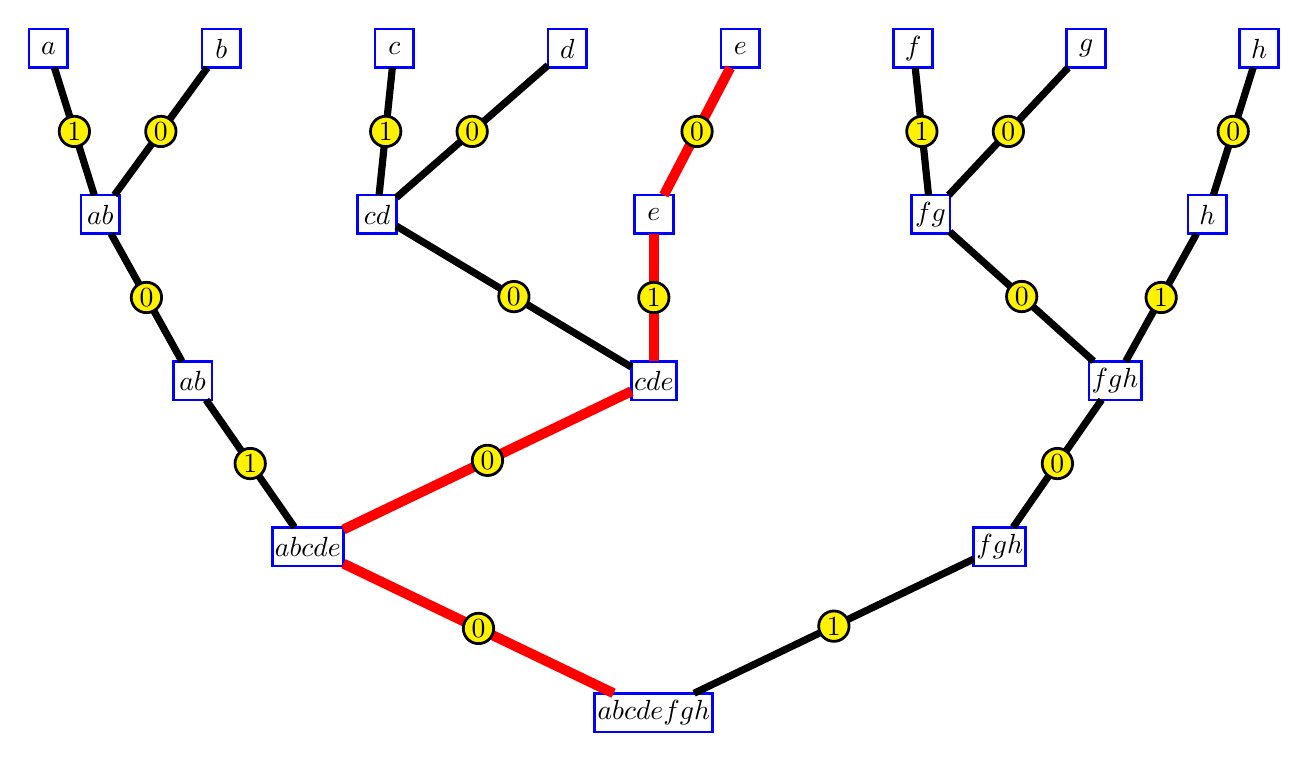
\begin{tikzpicture}[x=10pt,y=6pt]
  \centering
  \tikzset{VertexStyle/.style = {
    shape         = rectangle,
    draw          = blue, 
    fill          = white, 
  	line width    = 1pt, 
    text          = black,
    inner sep     = 1pt,
    outer sep     = 0pt,
    minimum size  = 14 pt,
    scale         = 1
    }
  }
  \tikzset{EdgeStyle/.style = {
    draw            = black, 
    thick,
    double          = black,
    double distance = 1pt
    }
  }
  \tikzset{RedEdgeStyle/.style = {
    draw            = red, 
    thick,
    double          = red,
    double distance = 2pt
    }
  }
  \tikzset{EdgeLabelStyle/.style = {
    draw          = black,
  	shape         = circle, 
  	line width    = 1pt, 
  	minimum size  = 10pt, 
    inner sep     = 1pt,
    outer sep     = 0pt,
    fill          = yellow,
    text          = black,
    scale         = 1
    }
  }

	\node[VertexStyle](A1) at (25, 0) {$abcdefgh$};
	\node[VertexStyle](B1) at (12.5, 10) {$abcde$};
	\node[VertexStyle](B2) at (37.5, 10) {$fgh$};
	\node[VertexStyle](C1) at (8.33333333333333, 20) {$ab$};
	\node[VertexStyle](C2) at (25, 20) {$cde$};
	\node[VertexStyle](C3) at (41.6666666666667, 20) {$fgh$};
	\node[VertexStyle](D1) at (5, 30) {$ab$};
	\node[VertexStyle](D2) at (15, 30) {$cd$};
	\node[VertexStyle](D3) at (25, 30) {$e$};
	\node[VertexStyle](D4) at (35, 30) {$fg$};
	\node[VertexStyle](D5) at (45, 30) {$h$};
	\node[VertexStyle](E1) at (3.125, 40) {$a$};
	\node[VertexStyle](E2) at (9.375, 40) {$b$};
	\node[VertexStyle](E3) at (15.625, 40) {$c$};
	\node[VertexStyle](E4) at (21.875, 40) {$d$};
	\node[VertexStyle](E5) at (28.125, 40) {$e$};
	\node[VertexStyle](E6) at (34.375, 40) {$f$};
	\node[VertexStyle](E7) at (40.625, 40) {$g$};
	\node[VertexStyle](E8) at (46.875, 40) {$h$};
	\draw[RedEdgeStyle](A1) to node[EdgeLabelStyle]{$0$} (B1);
	\draw[EdgeStyle](A1) to node[EdgeLabelStyle]{$1$} (B2);
	\draw[EdgeStyle](B1) to node[EdgeLabelStyle]{$1$} (C1);
	\draw[RedEdgeStyle](B1) to node[EdgeLabelStyle]{$0$} (C2);
	\draw[EdgeStyle](B2) to node[EdgeLabelStyle]{$0$} (C3);
	\draw[EdgeStyle](C1) to node[EdgeLabelStyle]{$0$} (D1);
	\draw[EdgeStyle](C2) to node[EdgeLabelStyle]{$0$} (D2);
	\draw[RedEdgeStyle](C2) to node[EdgeLabelStyle]{$1$} (D3);
	\draw[EdgeStyle](C3) to node[EdgeLabelStyle]{$0$} (D4);
	\draw[EdgeStyle](C3) to node[EdgeLabelStyle]{$1$} (D5);
	\draw[EdgeStyle](D1) to node[EdgeLabelStyle]{$1$} (E1);
	\draw[EdgeStyle](D1) to node[EdgeLabelStyle]{$0$} (E2);
	\draw[EdgeStyle](D2) to node[EdgeLabelStyle]{$1$} (E3);
	\draw[EdgeStyle](D2) to node[EdgeLabelStyle]{$0$} (E4);
	\draw[RedEdgeStyle](D3) to node[EdgeLabelStyle]{$0$} (E5);
	\draw[EdgeStyle](D4) to node[EdgeLabelStyle]{$1$} (E6);
	\draw[EdgeStyle](D4) to node[EdgeLabelStyle]{$0$} (E7);
	\draw[EdgeStyle](D5) to node[EdgeLabelStyle]{$0$} (E8);

  \end{tikzpicture}

\end{document}
